\chapter{Introducing MATSim}
\label{ch:introducing}
% ##################################################################################################################
\hfill \textbf{Author:} Kay W. Axhausen, Andreas Horni, ...

\begin{center} 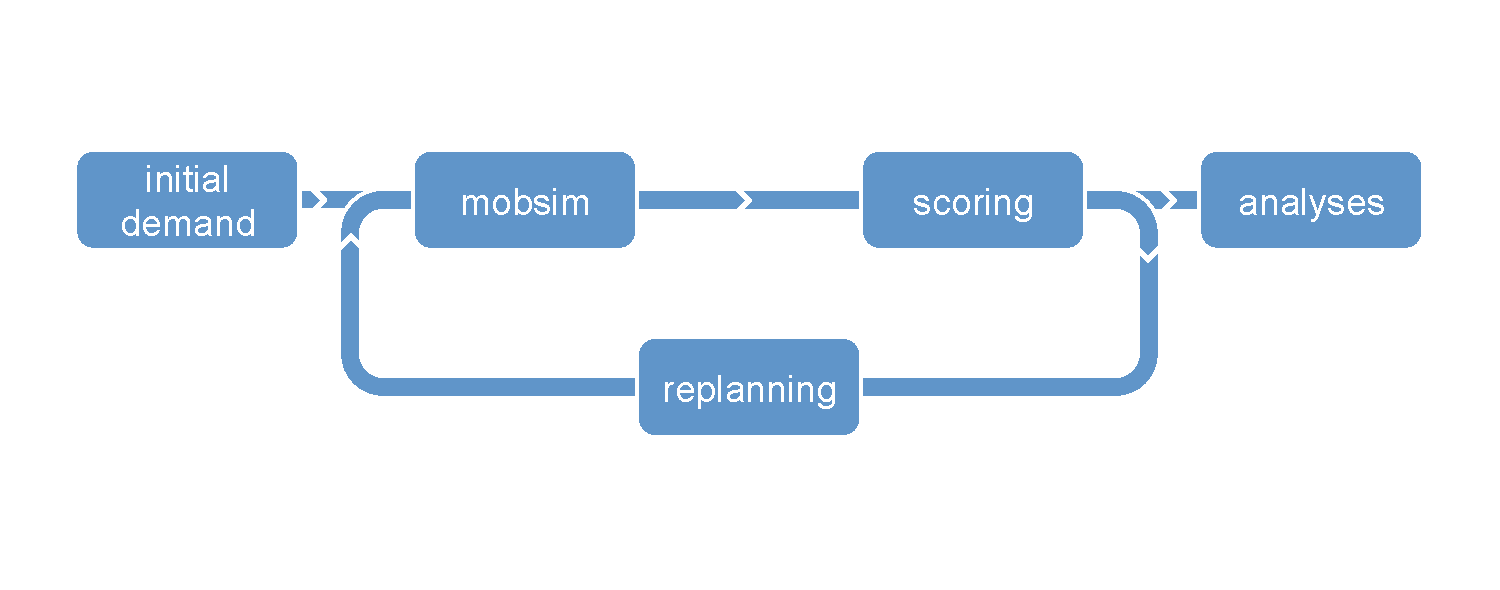
\includegraphics[width=0.7\textwidth, angle=0]{figures/matsimcycle.pdf} \end{center}

% ##################################################################################################################

%\ah{The development of the multi-agent transport simulation MATSim \citep[][]{MATSIM-T_Webpage_2014, BalmerEtAl_TRR_2006} has started approximately a decade ago as a collaborative effort of Prof.\ Nagel (now: TU Berlin) and Prof.\ Axhausen (ETH Zurich). It has its roots in \citet[][]{Axhausen_PhDThesis_1988} and in the transport simulation TRANSIMS \citep[][]{RaneyEtAl_LNCS_2002}, which was developed by Prof.\ Nagel as research team leader at the Los Alamos National Laboratory.}

% ##################################################################################################################
\section{How It Started}
The multi-\gls{agent} transport simulation MATSim \citep[][]{MATSIM-T_Webpage_2014} started with the wish of Kai~Nagel, then at ETH Zurich, to improve on his work with and for the TRANSIMS project \citep[][]{SmithEtAl_NTRPAC_1995} and to make the resulting code open-source. His background in traffic flow, complex adaptive systems, and large scale computation was complemented with experience in the agent-based modeling of travel demand when after Kai~Nagel's departure to Berlin in 2004 Kay~W.~Axhausen joined the effort in earnest. 

%\kai{Besteht jemand auf den ``Prof'' in obigem Text?  In wissenschaftlichen Texten m.E.\ eher unüblich.}
%\ah{Habs rausgenommen.}

It is this merger of two, actually three large and old streams of research, which has made the system unique from the start: 
\begin{compactitem}
\item microscopic description of demand by \emph{tracing the daily schedule} and the decisions involved of the agents modeled, 
%
\item integral microscopic \emph{simulation of the resulting traffic flows} and the resulting congestion (see Section~\ref{sec:trafficflowmodel}), and
%
\item  \emph{optimization of the experienced utilities} of the whole schedule through the co-evolutionary search for the resulting equilibrium or steady state (see Section~\ref{sec:co-ev}). 
%
\end{compactitem}
The robustness of this framework for the description of all congested spatial behaviors became clear, as the development progressed to include the congestion inside facilities and buildings or as parking was added. 

Agent-based modeling had been the basis of traffic flow simulation from the start in the 1970’s, e.g., \citet[][]{Wiedemann_PhDThesis_1974} or \citet[][]{Seddon_Simulation_1972}, but the work on traffic flow limited itself to individual links or small sequences of links and could therefore not address equilibrium as the aggregate assignment models could do from the 1970’s onward \citep[see][]{OrtuzarWillumsen_2011}. The expansion to whole and large networks came with the increasingly more powerful computers in the 1980’s and fast and accurate enough flow models (e.g.\ \citet[][]{NagelSchreckenberg_JdPI_1992, Schwerdtfeger_VolmulerHamerslag_1984, Daganzo_TransResPartB_1994}), but these agent-based simulations were not used to find an equilibrium at first. 

Agent-based modeling of travel demand had been developed in Germany \citep[][]{AxhausenHerz_JTE_1989}, but then also in English speaking countries after the seminal book of \citet[][]{JonesEtAl_1983}.  \kai{Da steht ``then'', aber das Datum bei Jones ist deutlich früher. ??}  While the Anglophone authors focused on sample enumeration methods to estimate the total demand with their agent-based demand models (\citet[see][]{BradleyBowman_TRBTDF_2006} for the North American, mostly discrete choice model based, developments, and \citet[][]{ArentzeTimmermans_2000} for an alternative Dutch approach), the simpler German approach was linked with an integral mesoscopic traffic flow simulation in \citet[][]{Axhausen_PhDThesis_1988}, but not used for equilibrium search. It had already a simple description of the total utility of the daily schedule.

\kai{according to Russel and Norvig, an agent is ``something that perceives and acts''.  Ich würde insbesondere ``perception'' bei fast allen der Arbeiten oben bezweifeln.  Außer vielleicht bei Wiedemann, aber dort richtet sich die Perzeption auch auf einen anderen Aspekt (nämlich driving). Darf ich durch die Absätze nochmal durchgehen und sie etwas abschwächen/differenzieren?}

Nash-equilibrium like approaches had been developed in transport assignment since the seminal \citet[][]{Wardrop_PICE_1952} paper, these aggregate flow based approaches were expanded to account for perception errors of the user and for the social optimum \citep[see][]{DaganzoSheffi_TransScience_1977}, but their reformulation for an disaggregate agent-based solution had to wait until the late 1990’s with \citet[][]{Gawron_IJMPC_1998} and TRANSIMS \citep[][]{SmithEtAl_NTRPAC_1995}. These approaches translated the logic of genetic algorithms into co-evolutionary search scheme, which efficiently identified the optima of each agent’s daily schedule.

At the end of 1990’s the scene was set for a merger of these strands into a computationally efficient, modular and open-source software enabling further development on travel behavior, network response and efficient computation. 

As shown on the web page \citep[][]{MATSIM-T-Scenarios_Webpage_2015} and detailed in Chapter \ref{ch:scenarios}, MATSim has been applied by local research groups world-wide for multiple different regions. \ah{see Discussion~\ref{sec:matsimtd}}

% ##################################################################################################################
\section{In Brief}
\label{sec:inbrief}
MATSim is an activity-based, extendable, multi-agent simulation framework 
%toolkit
%\kai{m.E.\ framework} 
implemented with the current version of the \gls{java}. It is open-source and can be downloaded at \citep[][]{MATSIM-T_Webpage_2015, SourceForge_Webpage_2015}. The framework is especially designed for large-scale scenarios, meaning that the features of all models are generally stripped down to efficiently handle the targeted functionality, where emphasis has been also been laid on parallelization \citep[e.g.,][]{Dobler_TechRep_IVT_2011, Charypar_PhDThesis_2008}. For the network loading simulation, for example, a queue-based model is implemented, leaving out the very complex and computationally expensive car-following behavior (see Section~\ref{sec:trafficflowmodel}).

For now, MATSim is conceptually designed to model a \emph{single day}, the common unit of analysis for activity-based models (see, for example, the review in \citet[][]{Bowman_TEC_2009_1}). In other words, MATSim is limited to the dynamics within that day. Nevertheless, in principle a multi-day model could be implemented \citep[][]{HorniEtAl_TechRep_IVT_2012_a}.

As shown in Section~\ref{sec:co-ev}, MATSim is based on the co-evolutionary principle. While being in a competition for space-time slots on the transportation infrastructure with all the other agents, every agent iteratively optimizes its daily \gls{activity} schedule. Figure~\ref{fig:matsimcycle} shows the iterative \index{MATSim loop}, whose details are explained below. 

% ------------
\createfigure%
{MATSim Cycle}%
{MATSim Cycle}%
{\label{fig:matsimcycle}}%
{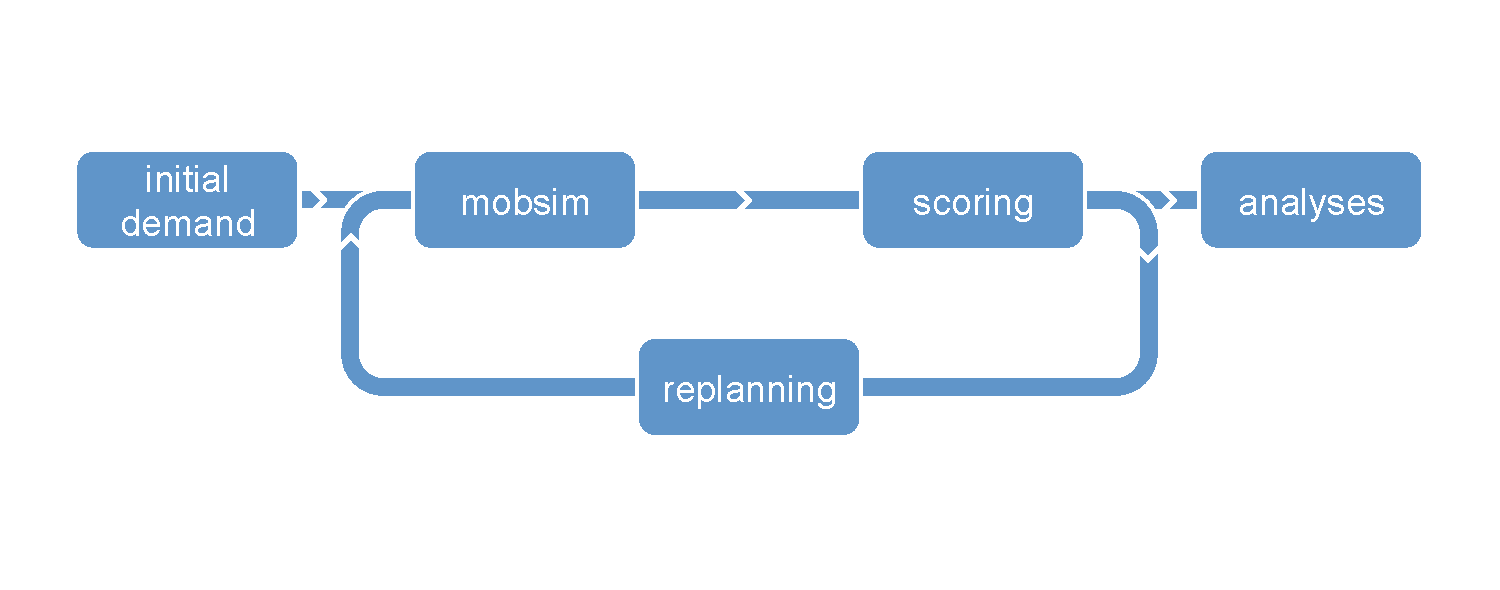
\includegraphics[width=0.99\textwidth, angle=0]{figures/matsimcycle.pdf}}%
{}
% ------------

MATSim starts with an initial demand, which arises from the study area population's daily activity chains. The modeled persons are called agents in MATSim. The activity chains are usually derived from empirical data through sampling or discrete choice modeling. A variety of approaches is suitable as can be seen in the scenarios' chapter (Chapter~\ref{ch:scenarios}). During the iterations this initial demand is optimized. Every agent possesses a memory of a fixed number of day plans, where each \gls{plan} is composed of a daily activity chain and an associated utility value (in MATSim called \emph{plan \gls{score}}).

In every iteration, prior to the simulation of the network loading with the MATSim \gls{mobsim} \citep[e.g.,][]{Cetin_PhDThesis_2005} (\emph{execution}), every agent selects a plan from its memory. This selection is dependent on the plan \gls{utility}. A certain share of the agents 
%$\varphi$ 
(often 10$\%$) is allowed to clone the selected plan and modify this clone (\emph{\gls{replanning}}). With the method of successive averages (MSA) usually a decreasing share of travelers is reallocated to a new plan to avoid oscillations. For MATSim, it has been shown that a variable replanning share over the course of the iterations can be productive and \emph{``increases overall performance of the system by a factor of three or more''} \citep[][p.7f]{CharyparEtAl_IATBR_2006}. For the network loading microsimulation step multiple simulations are available and configurable \citep[][p.10f]{HorniEtAl_TechRep_IVT_2011_a}. 

Plan modification is performed by the \emph{replanning} modules. Four dimensions are usually considered for MATSim at this time: departure time (and implicitly activity duration) \citep[][]{BalmerEtAl_Timmermans_2005}, route \citep[]{LefebvreBalmer_STRC_2007}, mode, and destination. Further dimensions such as activity adding or dropping or parking and group choices are currently under development and only available experimentally. % Siehe Tabelle MATSim-Präsentationen Prof.\ Axhausen.
MATSim replanning offers different strategies to adapt plans ranging from random mutation to approximate suggestions, to best response answers, where in every iteration the currently optimal choice is searched. Usually, routing and destination replanning are best response modifications, while time and mode replanning are random mutations. 

The initial day chains do not need to be very carefully defined for the replanning dimensions that are included in the optimization process. Plausible values just speed-up the optimization process. 

If an agent ends up with too many plans (configurable), the plan with the lowest score (configurable) is removed from the memory of this agent. The agents that have not undergone replanning select between existing plans. The selection model is configurable; in many MATSim investigations, a model that generates a logit distribution for plan selection is used.

An iteration is completed by evaluating the agents' day experience of the selected day plans (\emph{scoring}). The applied utility function is described in detail in Chapter \ref{ch:scoring}.

The iterative process is repeated until the average population score stabilizes, where the definition of the stopping criterion is subject of research initialized by \citet[][]{Meister_PhDThesis_2011, NagelFloetteroed_IATBR_2009}. The typical score development curve (Figure~\ref{fig:scoreprogress}, taken from \citet[][]{HorniEtAl_TRR_2009}) has the form of an evolutionary optimization progress \citep[][p.]{EibenSmithJE_2003}.

MATSim offers considerable customizability through its modular design. Although replacing core modules, such as the network loading simulation is associated with a substantial effort \citep[][Section 2.4]{MATSim_Userguide_2014}, in principle every module of the framework can be exchanged. MATSim modules are described in Chapter \ref{ch:modules} and following.

MATSim is heavily based on events. Every action in the simulation generates an event, which is recorded for analysis. These event records can be aggregated to evaluate any measure at the desired resolution. The event architecture is detailed in Section~\ref{sec:events-extension-point}.

% ------------
\createfigure%
{Typical Score Progress \kwaah{replace by single line plot}}%
{Typical Score Progress}%
{\label{fig:scoreprogress}}%
{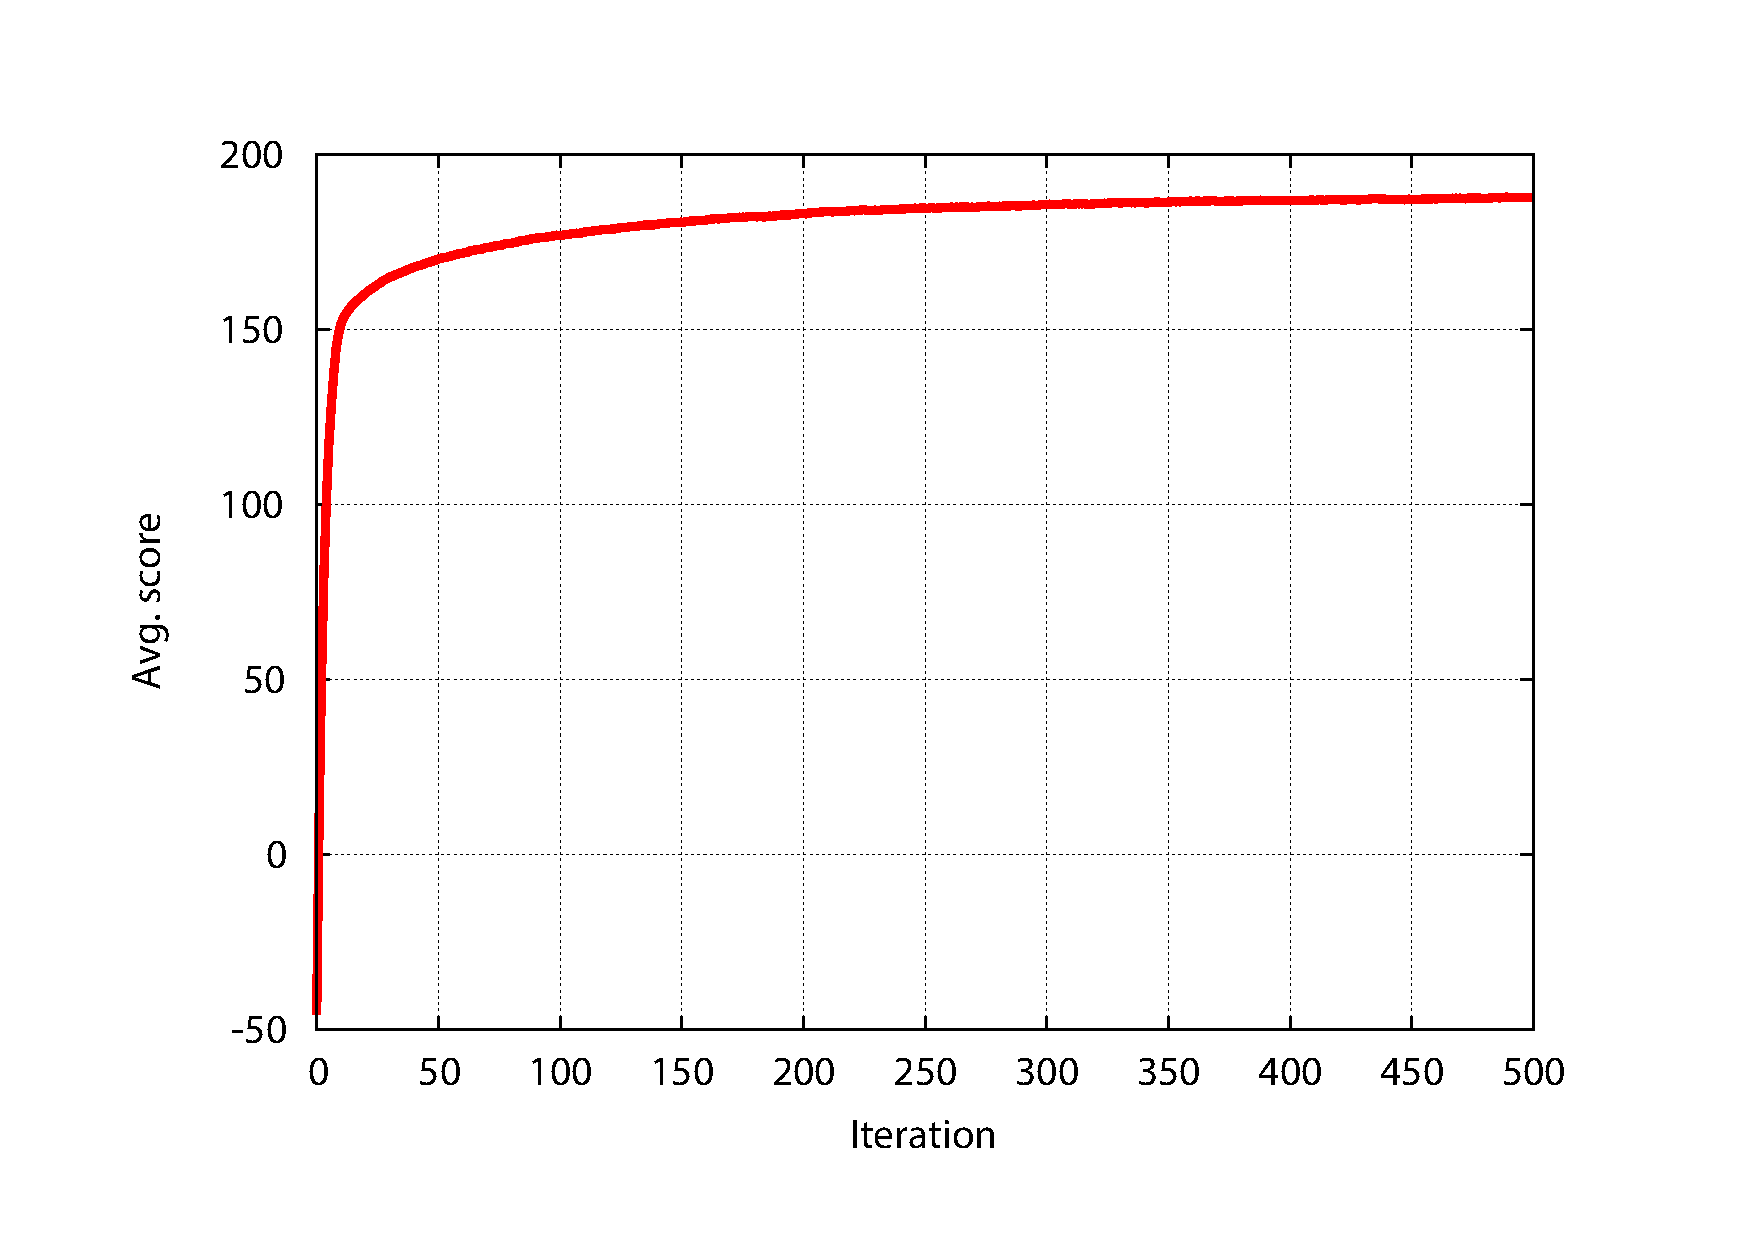
\includegraphics[width=0.99\textwidth, angle=0]{using/figures/scores.pdf}}%
{}
% ------------

% ##################################################################################################################
\section{MATSim's Traffic Flow Model}
\label{sec:trafficflowmodel}
MATSim provides two internal mobility simulations (called \emph{mobsims}): \emph{Qsim} and \emph{JDEQSim}. Furthermore, external mobility simulations can be plugged in. Some years ago the DEQSim written in C++ and described by \citet[][]{Charypar_PhDThesis_2008, CharyparEtAl_TRR_2007, CharyparEtAl_TRB_2009, CharyparEtAl_WCTRS_2007} was plugged into MATSim and frequently used. The multi-threaded Qsim is the default mobsim \citep[][]{MATSim_Userguide_2014}. % commit 29999 michaz

\citet[][]{CharyparEtAl_TRB_2009} distinguishes between 
\begin{compactitem}
\item physical microsimulation models, featuring detailed car following models,
\item cellular automata, in which roads are discretized into cells,
\item queue-based simulations, where traffic dynamics are modeled with waiting queues,
\item mesoscopic models, using aggregates to determine travel speeds, and
\item macroscopic models, based on flows rather than single traveler units (e.g., cars).
\end{compactitem}

As MATSim is designed for large-scale scenarios it adopts the computationally efficient queue-based approach (see Figure \ref{fig:queue}). A car entering a network link (i.e., a road segment) is added to the tail of the waiting queue. It remains there until the time for traveling the link with free flow has passed and until he or she is the head of the waiting queue and until the next destination link allows entering. The approach is very efficient, but clearly it comes at the price of reduced resolution, i.e., car following effects are not captured.   
%
\createfigure%
{Traffic Flow Model}%
{Traffic Flow Model}%
{\label{fig:queue}}%
{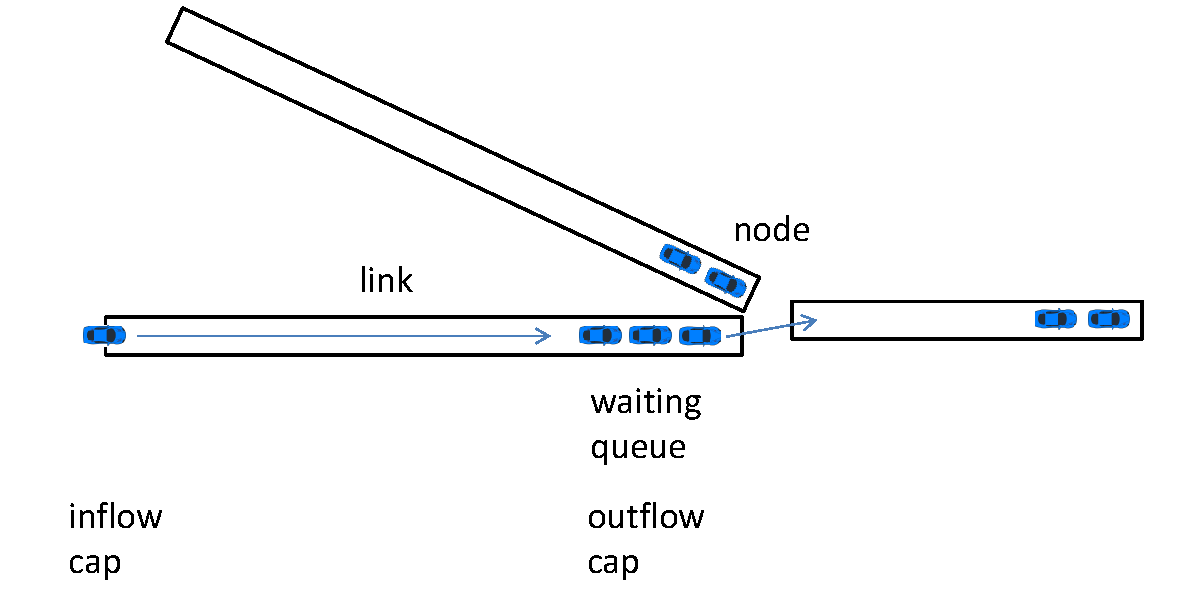
\includegraphics[width=0.99\textwidth, angle=0]{using/figures/queue.pdf}}%
{}
%
In JDEQSim, for computational reasons the waiting-queue approach is combined with an event-based update step \citep[][]{CharyparEtAl_TRB_2009}. In other words, there is no time-step-based updating process of any agent in the scenario. Instead agents are only touched if they actually require an action. For example, during the time an agent needs to pass a link (i.e., he or she is waiting in the queue), he or she does not need to be processed.  
%
%\kai{Ich kriege Ärger, wenn agents immer nur männlich sind.  Ist kein Witz; wurde mir bei meinen ersten öffentlichen Auftritten in Berlin sehr deutlich bedeutet.}  
% \ah{korrigiert}
Triggering of update events is managed by a global scheduler. 
QSim, however, is time-step based. \ah{see Discussion~\ref{sec:scenariod}}
%
%\kai{Aber in der QSim ist das nicht so; die ist ganz normal time-stepped.  Sie schaltet nur Kanten ab, die nicht ``aktiv'' sind.} 
%
% \ah{korrigiert}
%
The MATSim traffic flow model is heavily based on the two attributes of a link: storage capacity and flow capacity. Storage capacity defines the number of cars fitting onto a network link. It is a physical property and thus fixed in the simulation. 
%% For scenarios with a population smaller then the full population, say a 10\% sample, however, it needs to be scaled down, since otherwise there will be no spill-back any more.

Flow capacity specifies the outflow capacity of a link, i.e., how many travelers can leave the respective link. It is an individual attribute of the link. In the earlier DEQSim and in the current JDEQSim an additional inflow capacity can be specified in addition to capture breakdowns at link entries \citep[][p.99]{Charypar_PhDThesis_2008}. The many simulation experiments with Qsim (and the former queueSimulation) have shown that neglecting inflow capacity does not have a substantial effect but further reduces model complexity. 

This basic traffic flow model has been extended with various modules: signals and multiple lane modeling have been added (Chapter~\ref{ch:signalslanes}), backward-moving gaps as realized by \citet[][]{Charypar_PhDThesis_2008} are included in Qsim. Interactions between different modes are described in Chapter~\ref{ch:multimodalsim}. Limitations of the traffic flow model concern link dynamics (in particular overtaking and slow drivers) and intersection dynamics (in particular turn restrictions not explicitly modeled in the network). 


% ##################################################################################################################
\section{MATSim's Co-Evolutionary Algorithm}
\label{sec:co-ev}
%
% ------------
\createfigure%
{The Co-Evolutionary Algorithm in MATSim}%
{The Co-Evolutionary Algorithm in MATSim \kai{Nett.  Gibt es eine Quelle für den ``co-evolutionary algorithm''?} \ah{fürs Bild? Hab ich mir selber aus den Fingern gesogen. Für Co-EAs allgemein?} \thibaut{du kannst \cite{PopoviciEtAl_2012} gucken, find ich sehr gut. zum mindesten benutze ich immer diese in meine Papers}}%
{\label{fig:ea}}%
{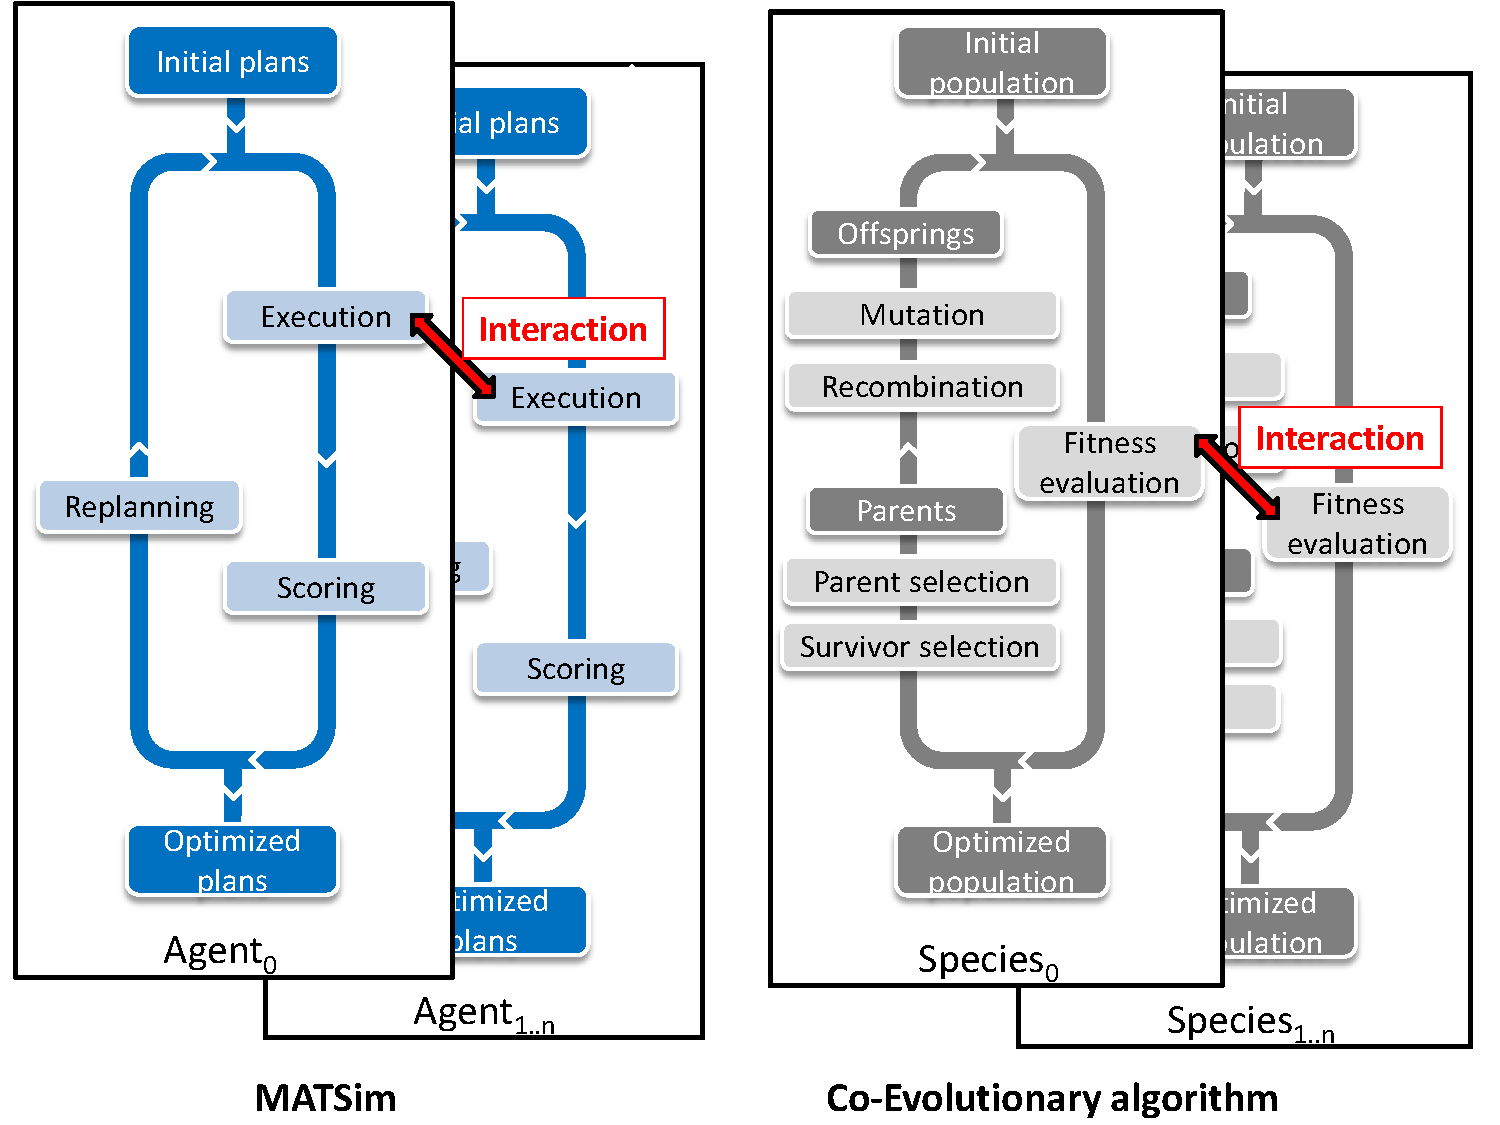
\includegraphics[width=0.99\textwidth, angle=0]{using/figures/MATSimVSea.pdf}}%
{}
% ------------
%
As illustrated in Figure \ref{fig:ea}, the MATSim equilibrium is searched by a \emph{\index{co-evolutionary algorithm}}. These algorithms co-evolve different species subject to interaction (e.g., competition). In MATSim, the individuals are represented by their plans, where a person represents a species. With the co-evolutionary algorithm, optimization is performed in terms of agents' plans , i.e.\ across the whole daily plan of activities and travel. It achieves more then the standard traffic flow equilibria, which ignore the activities. Eventually, an equilibrium is reached subject to constraints, where the agents cannot further improve their plans unilaterally. Strictly speaking, there is a difference between application of an evolutionary algorithm and a \emph{co}-evolutionary algorithm. An evolutionary algorithm would lead to a system optimum as optimization is applied with a global (or population) fitness function. The co-evolutionary algorithm instead leads to a (stochastic) user equilibrium as optimization is performed in terms of \emph{individual} utility functions and within an agent's set of plans. At the moment, the MATSim co-evolutionary algorithm only includes mutation; recombination may come into play when co-ordinated day plans of family members, for example, are included in the future.

% ##################################################################################################################
\section{Discussions}
% =============================================================================================
\subsection{MATSim-T, MATSim-F, MATSim}
\label{sec:matsimtd}

\kai{Wie gesagt, ich wäre gegen ``MATSim-T'' und für einfach nur ``MATSim''.  Siehe \url{http://matsim.org/conceptual-meeting/2012/notes}.}

\kai{
Bei einem der meetings (m.E. conceptual, aber es mach auch developer gewesen sein) gab es mal eine Diskussion, ob wir die Bezeichnung "toolbox" wirklich beibehalten wollen.

Wir waren uns damals einig, dass matsim eher ein framework als eine toolbox ist.

(ca. 30 vs. ca. 3 hits auf matsim.org)

Inzwischen, mit den "scripts-in-java", weicht das langsam ein wenig auf.  Aber wir hatten damals eigentlich beschlossen, sowohl auf "-T" als auch auf "-F" zu verzichten.

(Wir brauchen einen "Stadtschreiber", damit wir uns an solche Diskussionen erinnern. :-) )

Sollten wir das dann nicht auch im "Buch" machen?  Gibt es Personen, die an dem "-T" hängen?

}

% =============================================================================================
\subsection{Scenario}
\label{sec:scenariod}
\kwaah{We should add at the start that 'scenario' is the combination of case study data (population size, initial plans, networks and facilities), policies, the selected replanning modules and the selected traffic flow simulation.} 

\kai{I have to admit that I have that differently in my head.  
%
In the code, scenario is only the first, and this is also how I always had it in my own head: The ``XXX'' scenario is a collection of files.  
%
Selected replanning modules and selected traffic flow simulation is config; a sceanrio preferably comes together with a config that makes it runnable, but it is a different thing.  
%
And policy is policy; essentially the difference between (base case scenario | base case config) and (policy case scenario | policy case config).  
%
All three things together are a study for me.} 


\kai{Wobei ``scenario'' so wie hier im ursprünglichen Text benutzt m.E.\ stehen bleiben kann.}
%

\kwaah{
Kai, 

I have no problem either way, but see many text where the inclusive use is implied. 

But i am happy to see it split into 

Scenario: population plans networks facilities

Config = modules switched on

Policies

It is just that in many contexts in planning "Scenario" is equal to exeriment or run. If we are consistent fine

Kay
}

\kai{
oh weh.  So etwas wie "the considered policy scenario is the large-scale introduction of autonomous vehicles in Los Angeles County"? 

Vielleicht können wir 

(1) versuchen, "policy scenario" und "(matsim) scenario" erstmal auseinander zu halten

(2) es im Auge zu behalten, ob uns eine bessere Lösung einfällt.
%
...
%
Ich lese übrigens gerade nochmal (kleine) Teile des (großen) Buches von Russell/Norvig (Introduction to AI, a modern approach).  Da gibt es "utility based agents" ... 

... aber "An agent's utility function is essentially an internalization of the performance measure."

\textbf{\textit{Hier ist als "utility" nicht gleich "econometric utility"}}.
}


\kai{
Im Satz davor:

"a \textbf{performance measure} assigns a \textbf{score} to any given sequence of environment states"

Ein Unterschied scheint zu sein, dass das eher von außen gesehen wird, also das, was bei uns das Systemoptimum ist. 

Das liegt (m.E.) daran, dass "software agents" eher als Hilfsmittel zur Problemlösung gesehen werden; man versucht als, deren utility function so zu wählen, dass insgesamt der gewünschte Systemzustand rauskommt.

Hier weichen "agent-based systems" (im Sinne von mechanism design) also von "agent-based simulation" (im Sinne von "Modell der Wirklichkeit") voneinander ab.
}

\kwaah{
Danke, Kai

das sprachliche Monster ist ein Unding fuer den Alltag: (MATSim) scenario und policy run koennte vielleicht helfen. 

Die Frage nach score, utility, objective function ist genauso schwierig. Vielleicht sollten wir in den ersten beiden Teilen  von ‘score’ oder ‘objective function’ sprechen und erst in Teil 3 von utility

Kay
}

\gunnar{Ich weiss nicht, ob es hilft: Ich habe bislang "scenario" als "sufficient set of boundary conditions to execute the simulation" verstanden und "configuration" dann als dessen technische Spezifikation.
}

% ##################################################################################################################

% Local Variables:
% mode: latex
% mode: reftex
% mode: visual-line
% TeX-master: "../main"
% comment-padding: 1
% fill-column: 9999
% End: 
